\documentclass[11pt,]{article}
\usepackage[]{mathpazo}
\usepackage{amssymb,amsmath}
\usepackage{ifxetex,ifluatex}
\usepackage{fixltx2e} % provides \textsubscript
\ifnum 0\ifxetex 1\fi\ifluatex 1\fi=0 % if pdftex
  \usepackage[T1]{fontenc}
  \usepackage[utf8]{inputenc}
\else % if luatex or xelatex
  \ifxetex
    \usepackage{mathspec}
  \else
    \usepackage{fontspec}
  \fi
  \defaultfontfeatures{Ligatures=TeX,Scale=MatchLowercase}
\fi
% use upquote if available, for straight quotes in verbatim environments
\IfFileExists{upquote.sty}{\usepackage{upquote}}{}
% use microtype if available
\IfFileExists{microtype.sty}{%
\usepackage{microtype}
\UseMicrotypeSet[protrusion]{basicmath} % disable protrusion for tt fonts
}{}
\usepackage[margin=1in]{geometry}
\usepackage{hyperref}
\hypersetup{unicode=true,
            pdftitle={bluh},
            pdfauthor={Floor Komen},
            pdfkeywords={put some keywords here},
            pdfborder={0 0 0},
            breaklinks=true}
\urlstyle{same}  % don't use monospace font for urls
\usepackage{natbib}
\bibliographystyle{plainnat}
\usepackage{color}
\usepackage{fancyvrb}
\newcommand{\VerbBar}{|}
\newcommand{\VERB}{\Verb[commandchars=\\\{\}]}
\DefineVerbatimEnvironment{Highlighting}{Verbatim}{commandchars=\\\{\}}
% Add ',fontsize=\small' for more characters per line
\usepackage{framed}
\definecolor{shadecolor}{RGB}{248,248,248}
\newenvironment{Shaded}{\begin{snugshade}}{\end{snugshade}}
\newcommand{\KeywordTok}[1]{\textcolor[rgb]{0.13,0.29,0.53}{\textbf{#1}}}
\newcommand{\DataTypeTok}[1]{\textcolor[rgb]{0.13,0.29,0.53}{#1}}
\newcommand{\DecValTok}[1]{\textcolor[rgb]{0.00,0.00,0.81}{#1}}
\newcommand{\BaseNTok}[1]{\textcolor[rgb]{0.00,0.00,0.81}{#1}}
\newcommand{\FloatTok}[1]{\textcolor[rgb]{0.00,0.00,0.81}{#1}}
\newcommand{\ConstantTok}[1]{\textcolor[rgb]{0.00,0.00,0.00}{#1}}
\newcommand{\CharTok}[1]{\textcolor[rgb]{0.31,0.60,0.02}{#1}}
\newcommand{\SpecialCharTok}[1]{\textcolor[rgb]{0.00,0.00,0.00}{#1}}
\newcommand{\StringTok}[1]{\textcolor[rgb]{0.31,0.60,0.02}{#1}}
\newcommand{\VerbatimStringTok}[1]{\textcolor[rgb]{0.31,0.60,0.02}{#1}}
\newcommand{\SpecialStringTok}[1]{\textcolor[rgb]{0.31,0.60,0.02}{#1}}
\newcommand{\ImportTok}[1]{#1}
\newcommand{\CommentTok}[1]{\textcolor[rgb]{0.56,0.35,0.01}{\textit{#1}}}
\newcommand{\DocumentationTok}[1]{\textcolor[rgb]{0.56,0.35,0.01}{\textbf{\textit{#1}}}}
\newcommand{\AnnotationTok}[1]{\textcolor[rgb]{0.56,0.35,0.01}{\textbf{\textit{#1}}}}
\newcommand{\CommentVarTok}[1]{\textcolor[rgb]{0.56,0.35,0.01}{\textbf{\textit{#1}}}}
\newcommand{\OtherTok}[1]{\textcolor[rgb]{0.56,0.35,0.01}{#1}}
\newcommand{\FunctionTok}[1]{\textcolor[rgb]{0.00,0.00,0.00}{#1}}
\newcommand{\VariableTok}[1]{\textcolor[rgb]{0.00,0.00,0.00}{#1}}
\newcommand{\ControlFlowTok}[1]{\textcolor[rgb]{0.13,0.29,0.53}{\textbf{#1}}}
\newcommand{\OperatorTok}[1]{\textcolor[rgb]{0.81,0.36,0.00}{\textbf{#1}}}
\newcommand{\BuiltInTok}[1]{#1}
\newcommand{\ExtensionTok}[1]{#1}
\newcommand{\PreprocessorTok}[1]{\textcolor[rgb]{0.56,0.35,0.01}{\textit{#1}}}
\newcommand{\AttributeTok}[1]{\textcolor[rgb]{0.77,0.63,0.00}{#1}}
\newcommand{\RegionMarkerTok}[1]{#1}
\newcommand{\InformationTok}[1]{\textcolor[rgb]{0.56,0.35,0.01}{\textbf{\textit{#1}}}}
\newcommand{\WarningTok}[1]{\textcolor[rgb]{0.56,0.35,0.01}{\textbf{\textit{#1}}}}
\newcommand{\AlertTok}[1]{\textcolor[rgb]{0.94,0.16,0.16}{#1}}
\newcommand{\ErrorTok}[1]{\textcolor[rgb]{0.64,0.00,0.00}{\textbf{#1}}}
\newcommand{\NormalTok}[1]{#1}
\usepackage{graphicx,grffile}
\makeatletter
\def\maxwidth{\ifdim\Gin@nat@width>\linewidth\linewidth\else\Gin@nat@width\fi}
\def\maxheight{\ifdim\Gin@nat@height>\textheight\textheight\else\Gin@nat@height\fi}
\makeatother
% Scale images if necessary, so that they will not overflow the page
% margins by default, and it is still possible to overwrite the defaults
% using explicit options in \includegraphics[width, height, ...]{}
\setkeys{Gin}{width=\maxwidth,height=\maxheight,keepaspectratio}
\IfFileExists{parskip.sty}{%
\usepackage{parskip}
}{% else
\setlength{\parindent}{0pt}
\setlength{\parskip}{6pt plus 2pt minus 1pt}
}
\setlength{\emergencystretch}{3em}  % prevent overfull lines
\providecommand{\tightlist}{%
  \setlength{\itemsep}{0pt}\setlength{\parskip}{0pt}}
\setcounter{secnumdepth}{0}
% Redefines (sub)paragraphs to behave more like sections
\ifx\paragraph\undefined\else
\let\oldparagraph\paragraph
\renewcommand{\paragraph}[1]{\oldparagraph{#1}\mbox{}}
\fi
\ifx\subparagraph\undefined\else
\let\oldsubparagraph\subparagraph
\renewcommand{\subparagraph}[1]{\oldsubparagraph{#1}\mbox{}}
\fi

%%% Use protect on footnotes to avoid problems with footnotes in titles
\let\rmarkdownfootnote\footnote%
\def\footnote{\protect\rmarkdownfootnote}

%%% Change title format to be more compact
\usepackage{titling}

% Create subtitle command for use in maketitle
\newcommand{\subtitle}[1]{
  \posttitle{
    \begin{center}\large#1\end{center}
    }
}

\setlength{\droptitle}{-2em}

  \title{bluh}
    \pretitle{\vspace{\droptitle}\centering\huge}
  \posttitle{\par}
    \author{Floor Komen}
    \preauthor{\centering\large\emph}
  \postauthor{\par}
      \predate{\centering\large\emph}
  \postdate{\par}
    \date{15 januari 2019}

\usepackage{booktabs}
\usepackage{longtable}
\usepackage{array}
\usepackage{multirow}
\usepackage[table]{xcolor}
\usepackage{wrapfig}
\usepackage{float}
\usepackage{colortbl}
\usepackage{pdflscape}
\usepackage{tabu}
\usepackage{threeparttable}
\usepackage{threeparttablex}
\usepackage[normalem]{ulem}
\usepackage{makecell}

\begin{document}
\maketitle
\begin{abstract}
Put the abstract over here
\end{abstract}

\section{2. Multiple linear
regression}\label{multiple-linear-regression}

In this chapter multiple linear models are generated. The demographics
tested in this model are the highly educated fraction in a municipality
\texttt{High\_educated\_frac}, the urban index of a municipality
\texttt{Urban\_index}, the mean income of the municipality
\texttt{Mean\_income}, the non-west factor \texttt{Non\_west} and the
fraction that is 60 plus in the municipality \texttt{Frac\_60plus}. The
error assumptions are also discussed. This are assumptions made for the
residuals, to check if meet the requirements for correct linear
regressions. These assumptions are: * Linearity: The expected value of
the error is zero * Constant variance: The variance of the error is
constant * Normality: The errors are normally distributed * Indepence:
The observations are sampled indipendently

\subsection{First model}\label{first-model}

The first model will be the model with all the demographics:\\
\(Y_i = \beta_0 + \beta_1*high educated fraction + \beta_2*Urban index + \beta_3*Mean income + \beta_4*Non west2 +\beta_5*Non west3 + \beta_6*Frac 60plus + \epsilon i\)\\
The outcome of this model is shown below:

\begin{table}[ht]
\centering
\begin{tabular}{rrrrr}
  \hline
 & Estimate & Std. Error & t value & Pr() \\ 
  \hline
(Intercept) & 0.3381 & 0.0314 & 10.78 & 0.0000 \\ 
  High\_educated\_frac & -0.0864 & 0.0454 & -1.90 & 0.0576 \\ 
  Urban\_index & -0.0193 & 0.0041 & -4.69 & 0.0000 \\ 
  Mean\_income & -0.0015 & 0.0011 & -1.46 & 0.1453 \\ 
  Non\_west2 & -0.0223 & 0.0065 & -3.45 & 0.0006 \\ 
  Non\_west3 & -0.0455 & 0.0095 & -4.77 & 0.0000 \\ 
  Frac\_60plus & -0.5904 & 0.1494 & -3.95 & 0.0001 \\ 
   \hline
\end{tabular}
\end{table}

The first model is the total model, \texttt{high\_educated\_frac} and
\texttt{Mean\_income} do not have a significant t-value. Before any
conclusions are made, the assumptions are checked via plots and the VIF
is checked. The VIF is the Variation Inflation Factor, it implies if
there is multicollinearity between two or more variables. The formula
for VIF is \(1/(1-R^2)\) and the thresholdvalue is 10. So values above
10 give signs of multicollinearity. As shown below none of the values
are above 10, so no signs of collinearity.

\begin{verbatim}
##                        GVIF Df GVIF^(1/(2*Df))
## High_educated_frac 1.871032  1        1.367857
## Urban_index        3.383149  1        1.839334
## Mean_income        1.658015  1        1.287640
## Non_west           3.293503  2        1.347146
## Frac_60plus        1.289979  1        1.135772
\end{verbatim}

\begin{verbatim}
## [1]  74 298
\end{verbatim}

\begin{figure}[H]

{\centering 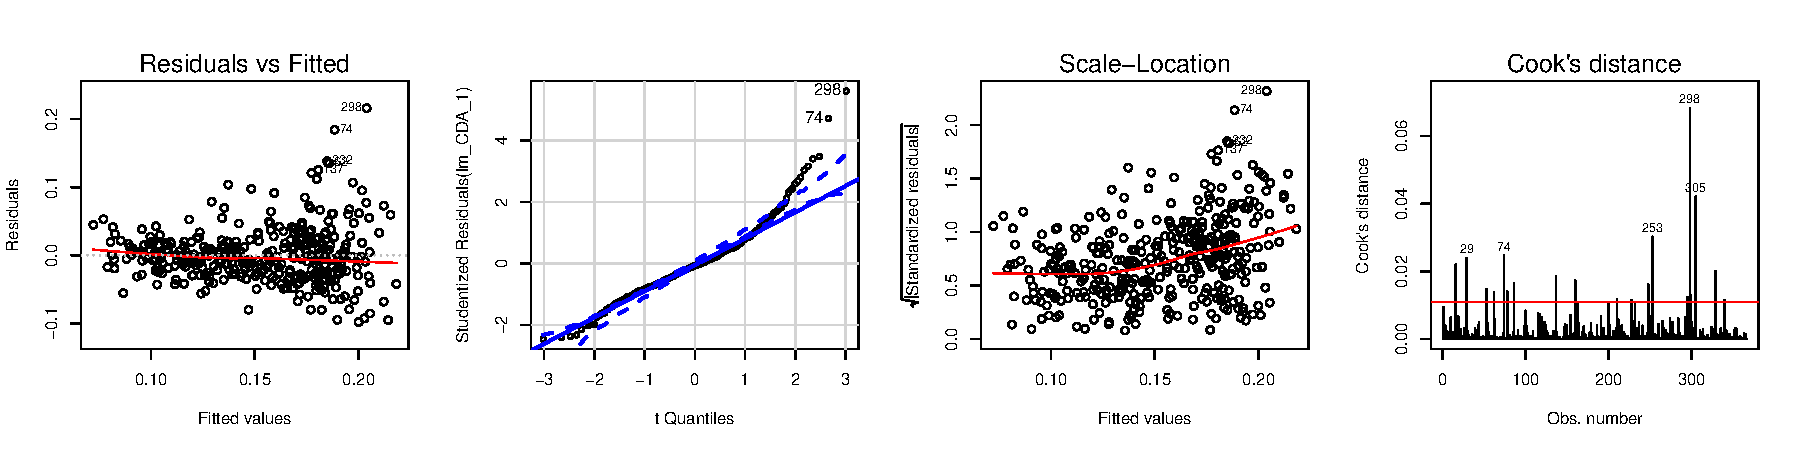
\includegraphics{lm_part_report_files/figure-latex/unnamed-chunk-1-1} 

}

\caption{\label{afm}assumptions first model}\label{fig:unnamed-chunk-1}
\end{figure}

In figure \ref{afm} the four plots are shown. The first plot (Residuals
vs Fitted) shows that the residuals have a `loudspeaker pattern', the
variance of the residuals tends to increase with an increase of the
fitted value. Because of this, a BoxCox graph is consulted. This graph
suggests a transformation for the response. The BoxCos figure \ref{BC1}
in has a 95\% Confidence interval located around the 0. So a ln
transformation is suggested.

\begin{figure}[H]

{\centering 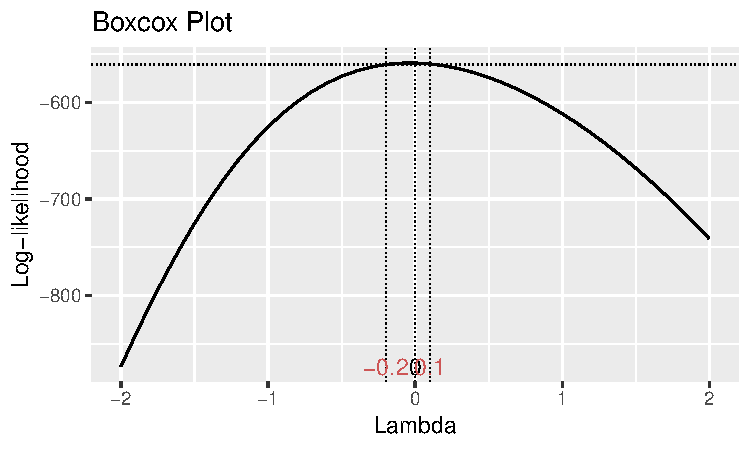
\includegraphics{lm_part_report_files/figure-latex/unnamed-chunk-2-1} 

}

\caption{\label{BC1}BoxCox first model}\label{fig:unnamed-chunk-2}
\end{figure}

\subsection{Second model}\label{second-model}

In the second model the response variable will be ln transformed. So the
new model will be:\\
\(ln(Y_i) = \beta_0 + \beta_1*high educated fraction + \beta_2*Urban index + \beta_3*Mean income + \beta_4*Non west2 + \beta_5*Non west 3 + \beta_6*Frac 60plus + \epsilon i\)

\begin{table}[ht]
\centering
\begin{tabular}{rrrrr}
  \hline
 & Estimate & Std. Error & t value & Pr() \\ 
  \hline
(Intercept) & -0.9944 & 0.1882 & -5.28 & 0.0000 \\ 
  High\_educated\_frac & -0.8808 & 0.2723 & -3.24 & 0.0013 \\ 
  Urban\_index & -0.1388 & 0.0247 & -5.62 & 0.0000 \\ 
  Mean\_income & -0.0024 & 0.0064 & -0.38 & 0.7042 \\ 
  Non\_west2 & -0.0991 & 0.0389 & -2.55 & 0.0112 \\ 
  Non\_west3 & -0.2763 & 0.0572 & -4.83 & 0.0000 \\ 
  Frac\_60plus & -2.6940 & 0.8965 & -3.01 & 0.0028 \\ 
   \hline
\end{tabular}
\end{table}

\begin{verbatim}
## [1]  16 237
\end{verbatim}

\begin{figure}[H]

{\centering 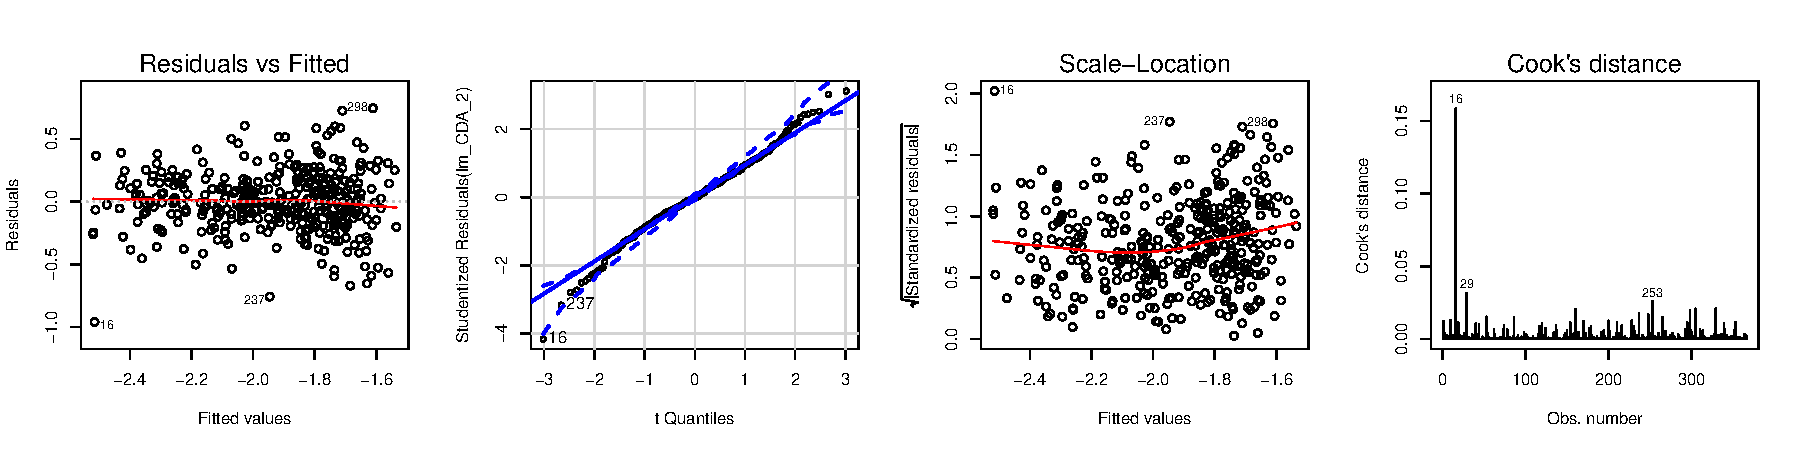
\includegraphics{lm_part_report_files/figure-latex/unnamed-chunk-3-1} 

}

\caption{\label{asm}assumptions second model}\label{fig:unnamed-chunk-3}
\end{figure}

The plots in figure \ref{asm} show one big outlier, the municipality
Amsterdam which has number 16. Amsterdams value for the cooks distance
goes way above the cutoff value for cooks, \(4/(369-5-1)=0.011\). It is
also outside the (-3,3) range with the studentized residuals. That is
why this municipality is removed.\\
For the second model without Amsterdam, a step function is used. This
step function uses the AIC for backward elimination. If the AIC can get
lower, because a variable is removed that variable will be removed else
no variable is removed. The formula for AIC is
\(AIC=-2log(likelihood)+2p\), p is the number of parameters in the
model. The variables that are left are the variables used in the final
model.

\begin{verbatim}
## Start:  AIC=-1041.5
## log(CDA_frac) ~ High_educated_frac + Urban_index + Mean_income + 
##     Non_west + Frac_60plus
## 
##                      Df Sum of Sq    RSS     AIC
## - Mean_income         1   0.04208 20.291 -1042.7
## <none>                            20.249 -1041.5
## - High_educated_frac  1   0.36195 20.611 -1037.0
## - Frac_60plus         1   0.67266 20.922 -1031.6
## - Non_west            2   1.54236 21.792 -1018.7
## - Urban_index         1   1.72696 21.976 -1013.6
## 
## Step:  AIC=-1042.74
## log(CDA_frac) ~ High_educated_frac + Urban_index + Non_west + 
##     Frac_60plus
## 
##                      Df Sum of Sq    RSS     AIC
## <none>                            20.291 -1042.7
## - Frac_60plus         1   0.66435 20.956 -1033.0
## - High_educated_frac  1   0.85427 21.146 -1029.7
## - Non_west            2   1.51164 21.803 -1020.5
## - Urban_index         1   1.68687 21.978 -1015.6
\end{verbatim}

\begin{verbatim}
## 
## Call:
## lm(formula = log(CDA_frac) ~ High_educated_frac + Urban_index + 
##     Non_west + Frac_60plus, data = Data_CDA[-16, ])
## 
## Coefficients:
##        (Intercept)  High_educated_frac         Urban_index  
##            -1.0298             -0.8277             -0.1311  
##          Non_west2           Non_west3         Frac_60plus  
##            -0.1141             -0.2871             -3.0168
\end{verbatim}

\subsection{Final model}\label{final-model}

The backward elimination gave the final model.\\
\(ln(Y_i) = \beta_0 + \beta_1*high educated fraction + \beta_2*Urban index + \beta_4*Non west2 + \beta_5*Non west 3 + \beta_6*Frac 60plus + \epsilon i\)
The coëfficients are given in the table below

\begin{table}[ht]
\centering
\begin{tabular}{rrrrr}
  \hline
 & Estimate & Std. Error & t value & Pr($>$$|$t$|$) \\ 
  \hline
(Intercept) & -1.0298 & 0.1365 & -7.54 & 0.0000 \\ 
  High\_educated\_frac & -0.8277 & 0.2129 & -3.89 & 0.0001 \\ 
  Urban\_index & -0.1311 & 0.0240 & -5.46 & 0.0000 \\ 
  Non\_west2 & -0.1141 & 0.0378 & -3.02 & 0.0027 \\ 
  Non\_west3 & -0.2871 & 0.0559 & -5.13 & 0.0000 \\ 
  Frac\_60plus & -3.0168 & 0.8799 & -3.43 & 0.0007 \\ 
   \hline
\end{tabular}
\end{table}

\begin{verbatim}
## 237 298 
## 236 297
\end{verbatim}

\begin{figure}[H]

{\centering 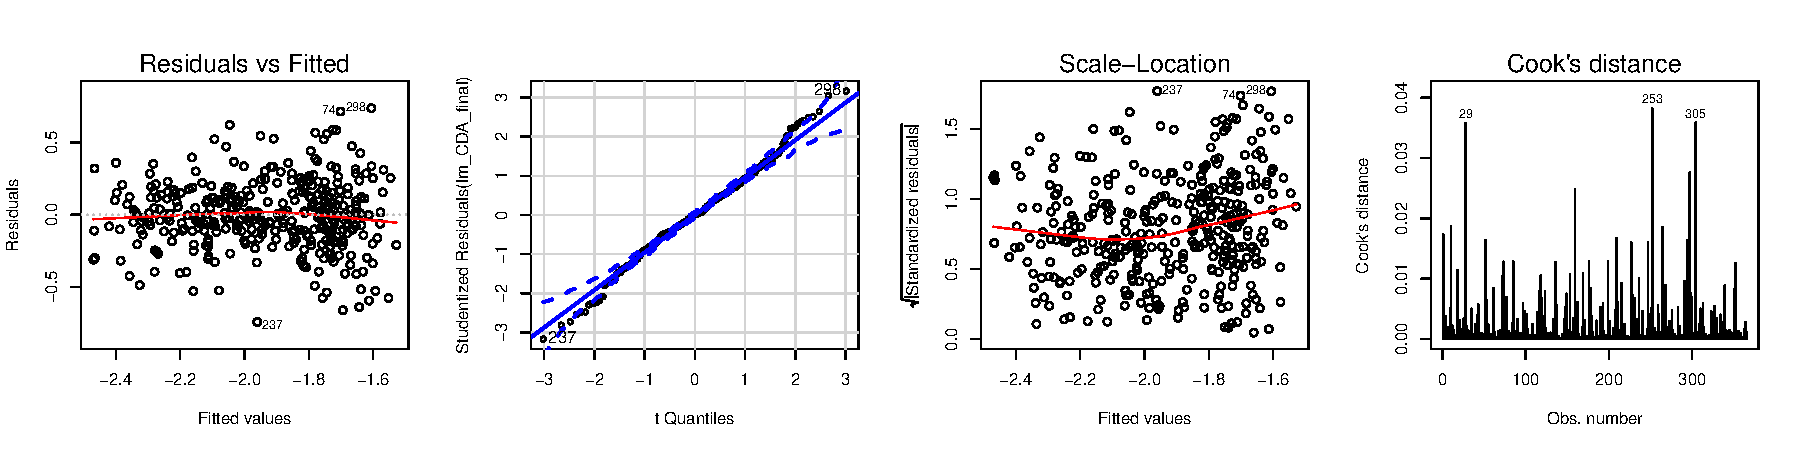
\includegraphics{lm_part_report_files/figure-latex/unnamed-chunk-5-1} 

}

\caption{\label{asm}assumptions second model}\label{fig:unnamed-chunk-5}
\end{figure}

The estimates for the predictors are filled in the model and the
following results are obtained:

\(ln(Y_i) = -1.0298 -0.8277*high educated fraction -0.1311*Urban index -0.1141*Non west2 -0.2871*Non west3 -3.0168*Frac 60plus + \epsilon i\)

All the coëfficients are negative, but because the fitted value is a log
value it will be positive.

\subsection{Cross validation}\label{cross-validation}

To tell something about the prediction possibilities of the model, cross
validation is done. Cross validation tells something about how well the
model predicts on average, it telss nothing about the 'correctness'of
the model. Cross validation estimates the expected prediction error of a
model.\\
The cross validation works as follows. First 5k-folds are made. This
means that the data is divided in five folds. Next, the loss function is
made. This function makes the square of the real value minues the
predicted value. By taking the sum of these values and the deviation by
amount of real values in the k-folds, the mean is taken. 4 of the 5
kfolds are used ase training data, the other one is the test/validation
data. The model is fitted on the training data and afterwards it tries
to fit on the test data, to see if it predicts closely. This is done 5
times, every time another fold is is the testdata. As is shown below,
the prediction error for this model is 0.0582

\begin{Shaded}
\begin{Highlighting}[]
\NormalTok{lm_CDA_final <-}\StringTok{ }\KeywordTok{lm}\NormalTok{(}\KeywordTok{log}\NormalTok{(CDA_frac) }\OperatorTok{~}\StringTok{ }\NormalTok{High_educated_frac }\OperatorTok{+}\StringTok{ }\NormalTok{Urban_index }\OperatorTok{+}\StringTok{ }\NormalTok{Non_west }\OperatorTok{+}\StringTok{ }
\StringTok{    }\NormalTok{Frac_60plus, }\DataTypeTok{data =}\NormalTok{ Data_CDA[}\OperatorTok{-}\DecValTok{16}\NormalTok{, ])}
\NormalTok{K <-}\StringTok{ }\DecValTok{5}
\NormalTok{index <-}\StringTok{ }\KeywordTok{rep}\NormalTok{(}\DecValTok{1}\OperatorTok{:}\NormalTok{K, }\KeywordTok{floor}\NormalTok{(}\KeywordTok{nrow}\NormalTok{(Data_CDA)}\OperatorTok{/}\NormalTok{K) }\OperatorTok{+}\StringTok{ }\DecValTok{1}\NormalTok{)[}\DecValTok{1}\OperatorTok{:}\KeywordTok{nrow}\NormalTok{(Data_CDA)]}
\NormalTok{fold.index <-}\StringTok{ }\KeywordTok{sample}\NormalTok{(index)}
\NormalTok{Loss <-}\StringTok{ }\ControlFlowTok{function}\NormalTok{(x, y) \{}
    \KeywordTok{sum}\NormalTok{((x }\OperatorTok{-}\StringTok{ }\NormalTok{y)}\OperatorTok{^}\DecValTok{2}\NormalTok{)}\OperatorTok{/}\KeywordTok{length}\NormalTok{(x)}
\NormalTok{\}}
\NormalTok{loss <-}\StringTok{ }\KeywordTok{numeric}\NormalTok{(K)}
\ControlFlowTok{for}\NormalTok{ (k }\ControlFlowTok{in} \DecValTok{1}\OperatorTok{:}\NormalTok{K) \{}
\NormalTok{    training <-}\StringTok{ }\NormalTok{Data_CDA[fold.index }\OperatorTok{!=}\StringTok{ }\NormalTok{k, ]}
\NormalTok{    validation <-}\StringTok{ }\NormalTok{Data_CDA[fold.index }\OperatorTok{==}\StringTok{ }\NormalTok{k, ]}
\NormalTok{    training.fit <-}\StringTok{ }\NormalTok{lm_CDA_final}
\NormalTok{    validation.predict <-}\StringTok{ }\KeywordTok{predict}\NormalTok{(training.fit, }\DataTypeTok{newdata =}\NormalTok{ validation, }\DataTypeTok{type =} \StringTok{"response"}\NormalTok{)}
\NormalTok{    loss[k] <-}\StringTok{ }\KeywordTok{Loss}\NormalTok{(}\KeywordTok{log}\NormalTok{(validation}\OperatorTok{$}\NormalTok{CDA_frac), validation.predict)}
\NormalTok{\}}
\KeywordTok{mean}\NormalTok{(loss)}
\end{Highlighting}
\end{Shaded}

\begin{verbatim}
## [1] 0.05814674
\end{verbatim}

\subsection{Discussion}\label{discussion}

\subsection{Linear regression}\label{linear-regression}

Because the fitted values are transformed to a ln form, it is also
possible to raise the coëfficients to a exponential power. The final
model obtained then is:

\(Y_i = e^(-1.0298 -0.8277*high educated fraction -0.1311*Urban index -0.1141*Non west2 -0.2871*Non west3 -3.0168*Frac 60plus + \epsilon i)\)

Per variable the influence will be discussed. The slope will start at
point exp(-1.0298), this is equal to 0.357. This means if all the other
demographic variables are zero, the fitted value will be equal to the
intercept, so equal to 0.357. This not a possible outcome, because a
Municipality with all these demographics equal to zero is no reality.
For the other coefficients it is a bit harder to predict there
influence, because of the log transformation and the different range the
different variables have. For example, the urban index has a 0-3.8 range
and education ahs a 0.12-0.47 range in this data set. But still some
remarks can be made about the slope of the model. The fraction 60 plus
has the lowest marginal impact on the slope, if everything else stays
the same an frac 60 plus changes for example 1 the exponent changes with
-3.02. The non west2 has the highest impact on the slope, because the
coëfficient is the lowest. Another important point is that or Non-west2
and Non-west3 are both zero, or Non-west2 is one ore Non west 3 is one.
The outcome of the crossvalidation for this model is 0.0582. So the mean
squared difference between the fitted and predicted value is 0.0582,
which is pretty close to 0. There are some limitations for this model,
because the response variable is a fraction and will never be larger
than one, theoratically a Generalized linear model would be better. Also
some assumptions are violated. In the fitted vs residual graph it is
visible that the variance is not equally spread, there is a small
``loudspeaker pattern''. But because the fitted values are log
transformed, it is not really possible to adapt this any further. Also
there are two municipalities that fall outside the {[}-3,3{]} range in
the normality plot, but because they are still in the 95\% envelope the
decision is made to not delete these municipalities.

\subsection{further research}\label{further-research}

Both of the models have different significant variables. But it is
difficult to say which one is a better fitting model. Because both of
them have reasons to choose that kind of model, also both of them have
limitations. That is why further research should be done to research
which of the model is the best fitting model. Another topic that can be
researched in further research is the influence of demographics on areas
of municipalities instead of whole municipialities. Because differences
between areas are nullified in the demographics of a municipality.

\subsection{Abstract}\label{abstract}

In this repport some demographics of dutch municipalities are compared
with the general Dutch election results of 2017. The demographic
variables in this research are the urban index, the fraction of high
educated persons in a municipality, the non west factor, a 1 for the
factor means less than 5\% non west residents, a 2 means 5 till 10\% non
west residents and a three means more than 10\% residents, the mean
income of the municipality and the fraction of persons who are 60 years
and older. The response variable is the CDA votes. Two models are made
to explain the influence of the demographics on the amount of votes for
CDA per municipality. The first model is a multiple linear model, the
fraction of CDA votes is the respons variable. Because of error
assumptions, the response variable is log transformed. The final model
with this transformation is:\\
\(Y_i = e^(-1.0298 -0.8277*high educated fraction -0.1311*Urban index -0.1141*Non west2 -0.2871*Non west3 -3.0168*Frac 60plus + \epsilon i)\)\\
The fraction 60 plus has the lowest marginal influence on the slope of
the model. The factor Non west2 has the highest marginal impact on the
slope. There are still some limitations, firstly because even though a
log transformation has been made there is still a non constant error
variance. Secondly because the respons variable is a fraction,
theoretically a generalized linear model would be better. That is why
the second kind of model described is a generalized linear model. HIER
GML SAMENVATTING PLUS DISCUSSION The final linear model has different
significant variables than the general linear model. It is difficult to
say which model is better, because both have there limitations. In
further research the best fitting model of those two can be obtained.


\end{document}
